%%%%%%%%%%%%%%%%%%%%%%%%%%%%%%%%%%%%%%%%%%%%%%%%%%%%%%%%%%%%%%%%%%%%%%%%%%%%%%%
%
% Introduction
% 
%%%%%%%%%%%%%%%%%%%%%%%%%%%%%%%%%%%%%%%%%%%%%%%%%%%%%%%%%%%%%%%%%%%%%%%%%%%%%%%


\chapter{Introduction}

\section{Granular Material}

\begin{figure}[H]
\subfloat[Hourglass]{
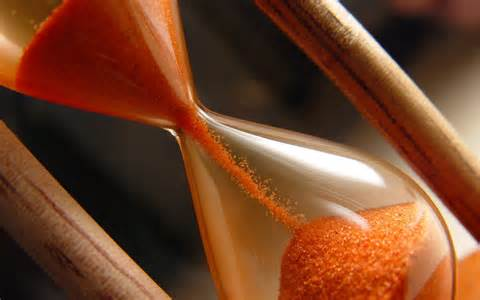
\includegraphics[width=0.5\textwidth]{../images/Intro/hourglass.jpg}
}
\subfloat[Heap of Sand]{
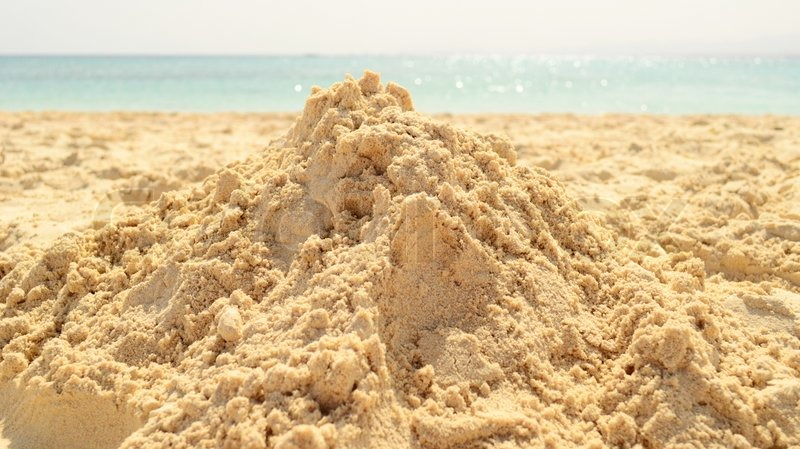
\includegraphics[width=0.5\textwidth]{../images/Intro/sand-heap.jpg}
}
\end{figure}

A granular material is a conglomeration of discrete solid, macroscopic particles characterized by a loss of energy whenever the particles interact (the most common example would be friction when grains collide). The constituents that compose granular material must be large enough such that they are not subject to thermal motion fluctuations. Thus, the lower size limit for grains in granular material is about 1$\mu m$. On the upper size limit, the physics of granular materials may be applied to ice floes where the individual grains are icebergs and to asteroid belts of the Solar System with individual grains being asteroids. \citep{duran}

Granular materials are very important in many industrial processes, in natural sciences and everyday life. A peculiar characteristic of granular materials is that, they behave differently under different circumstances. For example, they behave like fluids while flowing in an hour glass and pipes, whereas a heap of sand does not flow and behaves like a solid. The same heap of sand can deform plastically if some force is applied on it.

\section{Particle Simulations of Granulates}

\subsection{Why to simulate? }

\begin{figure}[H]
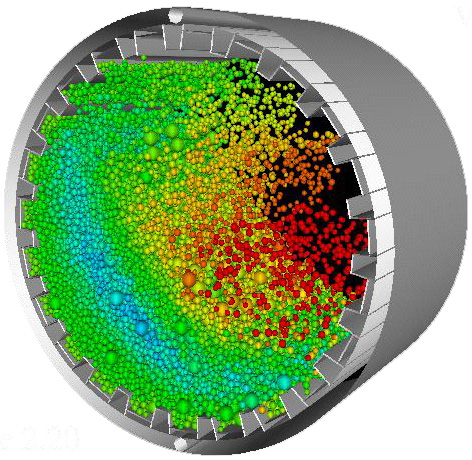
\includegraphics[scale=0.25]{../images/Intro/simulation.jpg}
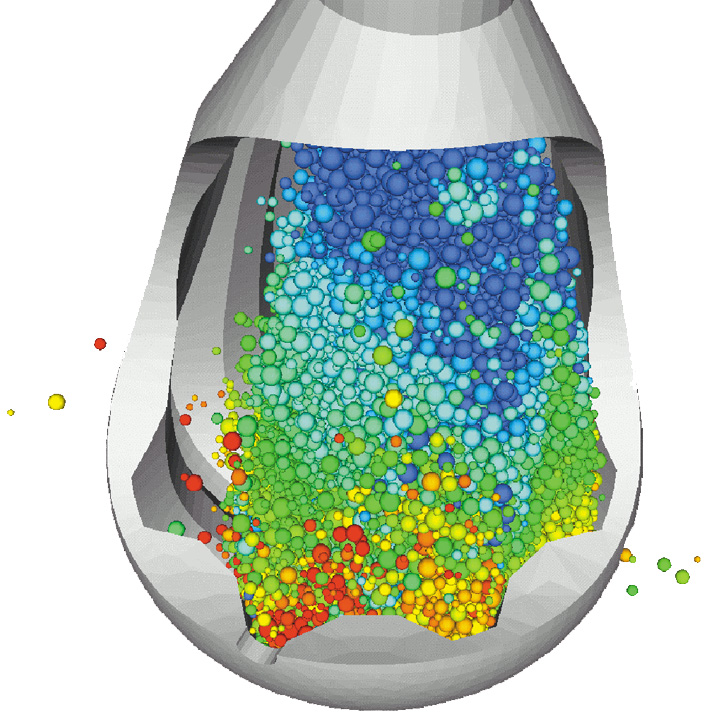
\includegraphics[scale=0.25]{../images/Intro/simulation1.jpg}
\end{figure}

There are many reasons to simulate granular materials \citep{por}. Conducting experiments with engineering devices are generally time consuming, dangerous and expensive, as they requires specialized equipment, They are extensively used in industries and are an important part of everyday life. Since there is no comprehensive theory on granular materials which reliable predict the behavior of such materials in technical devices, numerical simulations can be used to predict and to optimize the function of machinery in powder technology before the machine is built. Hence it makes sense to use the power of computers to simulate granular material.

\subsection{Methods of simulation}

A few of the models used in simulation of granular materials are

\subsubsection{Force Based Model}

In this model, the general idea is to solve numerically Newton's equations of motion.
\begin{itemize}
\item \textbf{Rigid Body dynamics}
The interaction forces are determined from consistency requirements on the behavior of the particles. This method is therefore suited to simulate perfectly rigid particles without the necessity to specify a certain deformation law.

\item \textbf{Molecular Dynamics}
In the most common version, the trajectories of granulates are determined by numerically solving Newton's equations of motion for a system of interacting granulates. Here the Newton's equation of motion is solved simultaneously for all particles $i$:
\begin{align*}
\ddot{\vec{r_{i}}} = \frac{1}{m_{i}} \vec{F_{i}}(\vec{r_{1}}, \vec{v_{1}},.....,\vec{r_{N}},\vec{v_{N}})
\end{align*}

\item \textbf{Discrete Element Method}

DEMs are closely related to Molecular Dynamics, but also includes rotational degrees-of-freedom as well as stateful contact and often complicated geometries. Discrete Elements methods are generally computationally intensive, therefore limiting the length of a simulation or number of particles.


\end{itemize}

\subsubsection{Event Driven Model}

In Event Driven Models, the flow of the algorithm is determined by events such as collisions in the case of simulation of granular materials. The trajectory and velocity of granulates after collisions is determined with factors such as coefficient of restitution.  


\section{Particle Models}

\subsubsection{Hertz Theory \citep{landau}}

The oldest and most influential model of contacts mechanics which can be used in force based models is the Hertz contact theory. In Hertz’s classical theory of contact, he focused primarily on non-adhesive contact where no tension force is allowed to occur within the contact area. The following assumptions are made in determining the solutions of Hertzian contact problems:

\begin{itemize}
\item The strains are small and within the elastic limit.
\item Each body can be considered an elastic half-space, i.e., the area of contact is much smaller than the characteristic radius of the body.
\item The surfaces are continuous and non-conforming.
\item The bodies are in frictionless contact.
\end{itemize}


\begin{figure}[H]
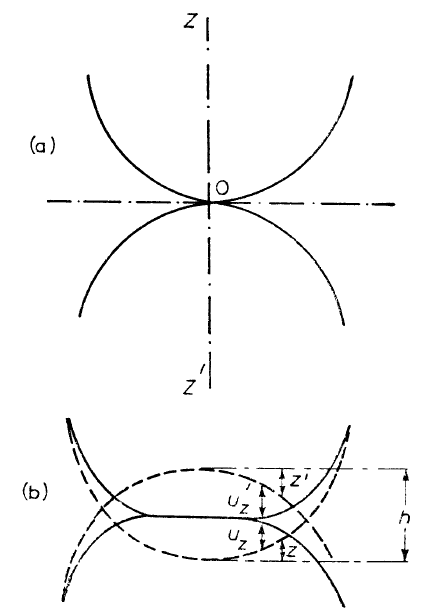
\includegraphics[scale=0.5]{../images/Intro/hertz.png}
\caption{Hertz Problem}
\label{fig:hertzfigure}
\end{figure}

Let two solid bodies be in contact at a point which is not a singular point on either surface. Figure \ref{fig:hertzfigure} shows a cross-section of the two surfaces near the point of contact $O$. The surfaces have a common tangent plane at $O$, which we take as the any-plane. We regard the positive z-direction as being into either body (i.e. in opposite directions for the two bodies) and denote the corresponding co-ordinates by $z$ and $z'$.

Near a point of ordinary contact with the xy—plane, the equation of the surface can be written

\begin{equation}
z = \kappa_{\alpha\beta}x_{\alpha}x_{beta}
\label{eq:contacteq1}
\end{equation}

where summation is understood over the values 1, 2, of the repeated suffixes $\alpha, \beta (x_{1} - x, x; = y)$, and $\kappa_{\alpha\beta}$ is a symmetrical tensor of rank two, which characterizes the curvature of the surface: the principal values of the tensor $\kappa_{\alpha\beta}$ are $\frac{1}{2R_{1}}$ and $\frac{1}{2R_{2}}$, where $R$ and $R_{2}$ are the principal radii of curvature
of the surface at the point of contact. A similar relation for the surface of the other body near the point of contact can be written

\begin{equation}
z' = \kappa'_{\alpha\beta}x_{\alpha}x_{beta}
\label{eq:contacteq2}
\end{equation}

Let us now assume that the two bodies are pressed together by applied
forces, and approach a short distance $h(Hertz’s problem)$. The deformation occurs near the original point of contact, and the two bodies will be in contact over a small but finite portion of their surfaces. Let $u$, and $u'$, be the components (along the $z$ and $z'$ axes respectively) of the corresponding displacement vectors for points on the surfaces of the two bodies. The broken lines in figure \ref{fig:hertzfigure} show the surfaces as they would be in the absence of any deformation, while the continuous lines show the surfaces of the deformed bodies; the letters $z$ and $z’$ denote the distances given by equations \ref{eq:contacteq1}
and \ref{eq:contacteq2}. It is seen at once from the figure that the equation

\begin{equation}
(z+u_{z}) + (z'+u') = h
\end{equation}

or 
\begin{equation}
(\kappa_{\alpha\beta}x_{\alpha}x_{beta} + \kappa'_{\alpha\beta}x_{\alpha}x_{beta})
\label{eq:contacteqcombined}
\end{equation}

holds everywhere in the region of contact. At points outside the region of
contact, we have

\begin{equation}
z+z'+u_{z}+u'_{z} > h
\end{equation}
We choose the x and y axes to be the principal axes of the tensor $\kappa_{\alpha\beta}+\kappa'_{\alpha\beta}$. Denoting the principal values of this tensor by $A$ and $B$, we can rewrite equation \ref{eq:contacteqcombined} as
\begin{equation}
Ax_{2}+By_{2}+u_{z}+u'_{z} = h
\label{eq:rewriteAB}
\end{equation}

We denote by $P_{z}(x,y)$ the pressure between the two deformed bodies at points in the region of contact; outside this region, of course $P_{z} = 0$. To determine the relation between $P_{z}$ and the displacements $u_{z}, u'_{z}$, we can with sufficient accuracy regard the surfaces as plane and use the formula \citep{landau}.
 
\begin{equation}
\begin{split}
u_{x} = \frac{1+\sigma}{2 \pi E} \frac{1}{r} \Big\{ -\frac{(1-2\sigma)x}{r}F_{z} + 2(1-\sigma)F_{x} + \frac{2\sigma x}{r^{2}} (xF_{x} + yF_{y}) \Big\} \\
u_{y} = \frac{1+\sigma}{2 \pi E} \frac{1}{r} \Big\{ -\frac{(1-2\sigma)y}{r}F_{z} + 2(1-\sigma)F_{y} + \frac{2\sigma y}{r^{2}} (xF_{x} + yF_{y}) \Big\} \\
u_{z} = \frac{1+\sigma}{2 \pi E} \frac{1}{r} \Big\{ 2(1-\sigma)F_{z} + \frac{2\sigma y}{r} (xF_{x} + yF_{y}) \Big\} \\
\end{split}
\label{eq:landau}
\end{equation}


\begin{equation}
u_{i} = \int\int G_{ik} (x - x', y-y', z) P_{k}(x',y') dx' dy'
\label{eq:landauu}
\end{equation}
According to the third of formulae \ref{eq:landau} and \ref{eq:landauu}, the
displacement u, under the action of normal forces $P_{z}(x, y)$ is given by

\begin{align}
\begin{split}
u_{z} = \frac{1-\sigma^{2}}{\pi E}\int\int\frac{P_{z}(x',y')}{r}dx'dy' \\
u'_{z} = \frac{1-\sigma'^{2}}{\pi E'}\int\int\frac{P_{z}(x',y')}{r}dx'dy' \\
\end{split}
\label{eq:normalpressure}
\end{align}

where $a, a'$ and $E, E'$ are the Poisson’s ratios and the Young’s moduli of the two bodies. Since $P = 0$ outside the region of contact, the integration extends only over this region. It may be noted that, from these formulae, the ratio $\frac{u_{z}}{u'_{z}}$ is constant:

\begin{equation}
\frac{u_{z}}{u'_{z}} = \frac{(1-\sigma^{2})E'}{(1-\sigma'^{2})E}
\label{eq:ratiodisplacement}
\end{equation}

The relations \ref{eq:rewriteAB} and \ref{eq:ratiodisplacement} together give the displacements in $u_{z}$, $u'_{z}$ at every point of the region of contact (although \ref{eq:normalpressure} and \ref{eq:ratiodisplacement}, of course, relate to
points outside that region also).

Substituting the expressions \ref{eq:normalpressure} in \ref{eq:rewriteAB}, we obtain

\begin{equation}
\frac{1}{\pi}\Big(\frac{1-\sigma^{2}}{E}+\frac{1-\sigma'^{2}}{E'}\Big)\int\int\frac{P_{z}(x',y')}{r}dx'dy' = h-Ax^{2}-By^{2}
\label{eq:pressuredistribution}
\end{equation}
This integral equation determines the distribution of the pressure $P_{z}$ over the region of contact. Its solution can be found by analogy with the following results of potential theory. The idea of using this analogy arises as follows:
firstly, the integral on the left-hand side of equation \ref{eq:pressuredistribution} is of type commonly found in potential theory, where such integrals give the potential of a
charge distribution; secondly, the potential inside a uniformly charged ellipsoid is a quadratic function of the co-ordinates.

If the ellipsoid $\frac{x^{2}}{a^{2}}+\frac{y^{2}}{b^{2}}+\frac{z^{2}}{c^{2}}$ is uniformly charged (with volume
charged density $\sigma$), the potential in the ellipsoid is given by


\begin{equation}
\phi(x,y,z) = \pi\sigma abc\int_{\infty}^{0} \Big\{ 1-\frac{x^{2}}{a^{2}+\xi} - \frac{y^{2}}{b^{2}+\xi} - \frac{z^{2}}{c^{2}+\xi} \Big\} \frac{d\xi}{\sqrt{(a^{2}+\xi)(b^{2}+\xi)(c^{2}+\xi)}}
\end{equation}
%

%%%%%%%%%
In the limiting case of an ellipsoid which is very much flattened in the $z$-direction $(c\rightarrow0)$. we have

\begin{equation}
\phi(x,y) = \pi\sigma abc\int_{\infty}^{0} \Big\{ 1-\frac{x^{2}}{a^{2}+\xi} - \frac{y^{2}}{b^{2}+\xi} \Big\} \frac{d\xi}{\sqrt{(a^{2}+\xi)(b^{2}+\xi)\xi}}
\end{equation}

in passing to the limit $(c\rightarrow0)$ we must of course put $z=0$ for points inside the ellipsoid. The potential $\phi(x,y,z)$ also be written as

\begin{equation}
\phi(x,y,z) = \int\int\int\frac{\rho dx'dy'dz'}{\sqrt{\{(x-x')^{2}+(y-y')^{2}+(z-z')^{2}\}}}
\end{equation}

where the integration is over the volume of the ellipsoid. In pasing to the limit $(c\rightarrow0)$, we must put $z=z'=0$ in the radicand; integrating over $z'$ between the limits

\begin{equation}
\pm c \sqrt{\{1-(\frac{x'^{2}}{a^{2}})-(\frac{y'^{2}}{b^{2}})\}}
\end{equation}
we obtain
\begin{equation}
\phi (x,y) = 2\rho c \int\int\frac{dx'dy'}{r}\sqrt{\Big(1-\frac{x'^{2}}{a^{2}} - \frac{y'^{2}}{b^{2}} \Big)}
\end{equation}
where
\begin{equation}
r = \sqrt{\{(x-x')^{2}+(y-y')^{2}\}}
\end{equation}
and the integration is over the area inside the ellipse

\begin{equation}
\frac{x'^{2}}{a^{2}} + \frac{y'^{2}}{b^{2}} = 1
\end{equation}
Equating the two expressions for $\phi(x,y)$, we obtain the identity

\begin{equation}
\int\int\frac{dx'dy'}{r}\sqrt{\Big( 1- \frac{x'^{2}}{a^{2} - \frac{y'^{2}}{b^{2}}} \Big)} = \frac{1}{2}\pi ab\int_{\infty}^{0} \Big( 1-\frac{x^{2}}{a^{2}+\xi} - \frac{y^{2}}{b^{2}+\xi} \Big) \frac{d\xi}{\sqrt{(a^{2}+\xi)(b^{2}+\xi)\xi}}
\label{eq:integrated_phi}
\end{equation}

Comparing this relation with equation \ref{eq:pressuredistribution}, we see that the right-hand sides are quadratic functions of $x$ and $y$ of the same foam, and the left-hand sides are integrals of the same form. We can therefore deduce immediately that the region of contact (i.e. the region of integration in \ref{eq:pressuredistribution}) is bounded
by an ellipse of the form

\begin{equation}
\frac{x^{2}}{a^{2}} + \frac{y^{2}}{b^{2}} = 1
\label{eq:ellipse}
\end{equation}


%%%%%%%%%


and that the function $P_{z}(x,y)$ must be of the form

\begin{equation}
P_{z}(x,y) = constant \times \sqrt{\Big( 1 - \frac{x^{2}}{a^{2}} - \frac{y^{2}}{b^{2}} \Big)}
\end{equation}


Taking the constant such that the integral $\int\int P_{z}dxdy$ over the region of
content is equal to the given total force $F$ which moves the bodies together.
we obtain

\begin{equation}
P_{z}(x,y) = \frac{3F}{2\pi ab} \sqrt{\Big( 1 - \frac{x^{2}}{a^{2}} - \frac{y^{2}}{b^{2}} \Big)}
\label{eq:contactforce}
\end{equation}

This formula gives the distribution of pressure over the tree of the region of
contact. It may be pointed out that the pressure at the centre of this region
is $\frac{3}{2}$ times the mean pressure $\frac{F}{\pi ab}$.

Substituting \ref{eq:contactforce} in equation \ref{eq:pressuredistribution} and replacing the resulting integral
in accordance with \ref{eq:integrated_phi}, we obtain

\begin{equation}
\frac{FD}{\pi} \int_{\infty}^{0} \Big( 1 - \frac{x^{2}}{a^{2} + \xi} - \frac{y^{2}}{b^{2} + \xi} \Big) \frac{d\xi}{\sqrt{(a^{2} + \xi)(b^{2} + \xi)\xi}} = h - Ax^{2} - By^{2}
\label{eq:D}
\end{equation}

where
\begin{equation*}
D = \frac{3}{4} \Big( \frac{1-\sigma^{2}}{E} + \frac{1-\sigma'^{2}}{E'} \Big)
\end{equation*}

This equation must hold identically for all values of $x$ and $y$ inside the ellipse \ref{eq:ellipse}; the coefficients of $x$ and $y$ and the free terms must therefore be respectively equal on each side. Hence we find

\begin{equation}
h = \frac{FD}{\pi} \int_{\infty}^{0} \frac{d\xi}{\sqrt{(a^{2} + \xi)(b^{2} + \xi)\xi}}
\label{eq:h}
\end{equation}

\begin{equation}
\begin{split}
A = \frac{FD}{\pi} \int_{\infty}^{0} \frac{d\xi}{(a^{2}+\xi)\sqrt{(a^{2} + \xi)(b^{2} + \xi)\xi}} \\
B = \frac{FD}{\pi} \int_{\infty}^{0} \frac{d\xi}{(b^{2}+\xi)\sqrt{(a^{2} + \xi)(b^{2} + \xi)\xi}}
\end{split}
\label{eq:freeterms}
\end{equation}

Equations \ref{eq:freeterms} determine the semi-axes $a$ and $b$ of the region of contact from the given force $F$ ($A$ and $B$ being known for given bodies). The relation \ref{eq:h} then gives the distance of approach h as a function of the force $F$. The right-hand sides of these equations involve elliptic integrals.

%%%%%%%%%


Thus the problem of bodies in contact can be regarded as completely
solved. The form of the surfaces (i.e. the displacements $u_{z}$, $u'_{z}$) outside the region of contact is determined by the same formulae \ref{eq:normalpressure} and \ref{eq:contactforce}; the values of the integrals can be found immediately from the analogy with the potential outside a charged ellipsoid. Finally, the formulae \ref{eq:landau} enable us to find also the deformation at various points in the bodies (but only, of course, at distances small compared with the dimensions of the bodies).

Let us apply these formulae to the case of contact between two spheres of
radii $R$ and $R'$. Here $A = B = \frac{1}{2R} + \frac{1}{2R'}$. It is clear from symmetry that $a = b$, i.e. the region of contact is a circle. From \ref{eq:freeterms} we find the radius $a$ of this circle to be

\begin{equation}
a = F^{\frac{1}{3}} \Big(\frac{DRR'}{R+R'} \Big)^{\frac{1}{3}}
\end{equation}

$h$ is in this case the difference between the sum $R+R’$ and the distance between the centres of the spheres. From \ref{eq:contactforce} we obtain the following relation between $F$ and $h$:

\begin{equation}
h = F^{\frac{1}{3}} \Big[ D^{2} \Big( \frac{1}{R} + \frac{1}{R} \Big) \Big]^{\frac{1}{3}}
\end{equation}

It should be noticed that $h$ is proportional to $F^{\frac{2}{3}}$; conversely, the force $F$ varies as $h^{\frac{3}{2}}$. We can write down also the potential energy $U$ of the spheres
in contact. Since $ -F = \frac{-\partial U}{\partial h}$, we have

\begin{equation}
U = h^{\frac{5}{2}} \frac{2}{5D} \sqrt{\frac{RR'}{R+R'}}
\label{eq:potential}
\end{equation}

Finally, it may be mentioned that a relation of the form $h = constant \times F^{\frac{2}{3}}$ or $F = constant \times h^{\frac{3}{2}}$, holds not only for spheres but also for other finite bodies in contact. This is easily seen from similarity arguments. If we make
the substitution

\begin{align*}
a^{2} \rightarrow \alpha a^{2}, \quad b^{2} \rightarrow \alpha b^{2}, \quad F \rightarrow \alpha^{\frac{3}{2}}F
\end{align*}
where $\alpha$ is an arbitrary constant, equations (9.12) remain  In
equation \ref{eq:h}, the right-hand side is multiplied by $\alpha$, and so $h$ must be replaced by $\alpha h$ if this equation is to remain unchanged. Hence it follows that $F$ must be proportional to $h^{\frac{3}{2}}$.



%%%%%%%%%
\subsubsection{Collision of two spheres}


Consider a system of coordinates in which the center of mass of the two spheres is at rest, the energy before the collision is equal to the kinetic energy of the relative motion $\frac{1}{2}mv^{2}$, where $v$ is the relative velocity of the colliding spheres and $\mu = \frac{m_{1}m_{2}}{m_{1} + m_{2}}$ their reduced mass. During the collision, the total energy is the sum of the kinetic energy, which may be written $\frac{1}{2}\mu h^{2}$, and the potential energy \ref{eq:potential}. By, the law of conservation of energy we have

\begin{equation}
\mu \Big( \frac{dh}{dt} \Big) ^{2} + kh^{\frac{5}{2}} = \mu v^{2}, \quad k=\frac{4}{5D}\sqrt{\frac{RR'}{R+R'}}
\label{eq:mass}
\end{equation}


The maximum approach $h_{0}$ of the spheres corresponds to the time when their relative velocity $h = 0$, and is $h_{0} = (\frac{\mu}{k})^{\frac{2}{5}} v^{\frac{4}{5}}$.
The time $\tau$ during which the collision takes place (i.e. $h$ varies from 0 to $h_{0}$ and back is

\begin{equation}
\tau = 2 \int_{h^{0}}^{0} \frac{dh}{\sqrt{v^{2} - \frac{kh^{\frac{5}{2}}}{\mu} }} = 2 \Big( \frac{\mu^{2}}{k^{2}v} \Big) ^{\frac{1}{5}} \int_{1}^{0} \frac{dx}{\sqrt{1-x^{\frac{2}{5}}}} = 2.94 \Big( \frac{\mu^{2}}{k^{2}v} \Big) ^{\frac{1}{5}}
\label{eq:time}
\end{equation}
 
By using the statical formulae obtained to solve the this problem, we have neglected elastic oscillations of the spheres resulting from the collision. If this is legitimate, the velocity $v$ must be small compared with the velocity of sound.


\subsubsection{Collision of a sphere with a rigid plane}

The case of a sphere colliding with a plane an be approximated as collision of two sphere, where one sphere has a radius of $\infty$ and mass also of $\infty$. Therefore using \ref{eq:time} with $m_{1}$ as mass of the sphere, $m_{2}=\infty$ as mass of the plane, $R_{1}$ as radius of the sphere and $R_{2}=\infty$ as radius of the plane.

Substituting $E'=\infty$ in \ref{eq:D}
\begin{align*}
D = \frac{3}{4} \Big( \frac{1 - \sigma}{E} \Big)
\end{align*}

From \ref{eq:mass} 
\begin{align*}
k &= \frac{4}{5D} \sqrt{\frac{R_{1} R_{2}}{R_{1} + R_{2}}}= \frac{4}{5D} \sqrt{\frac{R_{1}}{\frac{R_{1}}{R_{2}} + 1}}\\
k &= \frac{4}{5D} \sqrt{R_{1}} \\
k &= \frac{16E}{5(1-\sigma)} \sqrt{R_{1}}
\end{align*}

now $\mu=\frac{m_{1}m_{2}}{m_{1}+m_{2}}=m_{1}$

substituting the above values in \ref{eq:time} and considering $m_{1}=\frac{4}{3}\pi R_{1}^{3}$
\begin{align*}
\tau &= 2.94 \Big( \frac{\mu^{2}}{k^{2}v} \Big)^{\frac{1}{5}} \\
\tau &= 2.94R_{1}v^{\frac{1}{5}} \Big( \frac{5\pi \rho (1-\sigma)}{12E} \Big)^{\frac{2}{5}}
\end{align*}



\section{Aims}

The aim of this thesis is to check validity of quasi static assumptions by considering the collision of two spheres of same material and radius. The quasi-static approximation implies that
\begin{itemize}
\item The characteristic deformation rate is much smaller than the speed of sound in the system.
\item The microscopic relaxation time of the particle's material is negligibly small as compared to the duration of the impact.
\end{itemize}
One way to validate the approximations is by calculating the coefficient of restitution of the sphere. The coefficient of restitution would also give an idea of the conversion of kinetic energy to vibrations after impact is complete, which is ignored by the quasi static assumptions.
